\creaCapitulo{CUDA}

CUDA, siglas de \textit{Compute Unified Device Architecture} es una plataforma de computación paralela y un conjunto de APIs desarrollado por NVIDIA para ejecutar código general en sus GPUs. Incluye, entre otros, un modelo de programación a partir de C y C++; un compilador (\textit{nvcc}) que genera código tanto para CPU como para GPU; un entorno de ejecución un una API para gestionar memoria, lanzamientos de kernels, streams; y librerías construidas sobre el propio modelo. \cite{Kirk2010} La idea principal es permitir que el programador trate a la GPU como un dispositivo de cómputo masivamente paralelo.

A modo de referencia, los primeros trabajos en los que se utiliza una GPU para cómputo general aparecen a principios de los 2000, en 2004 se crea internamente CUDA, y se lanza oficialmente en 2007. Desde entonces, la evolución de CUDA ha ido ligada a la evolución propia de las GPUs de NVIDIA, manteniendo el modelo \textit{SIMT} y añadiendo unidades especializadas como \textit{Tensor Cores}, \textit{RT Cores}, o el mecanismo del \textit{Transformer Engine}. \cite{NVIDIA2026}

CUDA implementa un modelo SIMT (Single Instruction, Multiple Threads), en el cual el programador define un kernel (función \textit{\_\_global\_\_}) que se ejecuta en muchos hilos. Los hilos se agrupan en bloques, y los bloques en una grid, y cada bloque se ejecuta en un \textit{Streaming Multiprocessor}, dentro del cual los hilos se agrupan en warps de 32 hilos. \cite{Kirk2010} El warp es por tanto la unidad de ejecución con la que trabajamos.

Cuando se trabaja con CUDA se ha de tener en mente que se puede acceder a varias memorias diferentes, cada una con su propia latencia y ancho de banda, y entre ellas nos encontramos a los registros, que son la memoria de los hilos individuales, y la más rápida de todas; pasando por la memoria compartida (\textit{\_\_shared\_\_}), que usan los bloques; la memoria constante(\textit{\_\_constant\_\_}), que es de solo lectura, y va cacheada; y la memoria global, que se aloja en la VRAM de la GPU. \cite{Farber2011}

El rendimiento de la memoria dependerá del buen hacer del programador, que será el encargado de buscar la coalescencia en los accesos a memoria global, del uso del \textit{shared memory} para reutilizar datos, de que evite la divergencia de los warps, y de que se encargue de controlar los warps activos. 

La coalescencia ocurre cuando los 32 hilos de un warp acceden a direcciones de memoria que caen dentro de un mismo segmento continuo. \cite{Kirk2010} Esto permite que la GPU atienda todos esos accesos con una sola transacción de memoria, lo cual implica una mayor eficiencia en el kernel. 

Por otro lado, la divergencia de warps ocurre cuando los hilos de un mismo warp toman caminos distintos en una rama condicional. Como el warp ejecuta las instrucciones en modo SIMT, si los hilos divergen, el hardware debe serializar las rutas. \cite{Farber2011} Esto quiere decir que si los hilos se encuentran frente a un bloque if/else, lo que va a pasar es que el bloque if será ejecutado por los hilos que cumplan la condición, y el resto de hilos se quedarán en stand-by. A continuación, el resto de los hilos ejecutará el bloque else mientras los primeros se quedan esperando, y luego se combinarán los resultados.  

Hay un matiz importante a tener en cuenta a la hora de hablar de implementaciones CUDA, y es que esto que veremos aquí serán kernels, y no métodos de clase como anteriormente. Una forma de verlo es que tendremos clases (como \textit{Metodo}), y éstas tendrán sus métodos que accederemos de forma normal con un objeto de la clase, y por otro lado tendremos los kernel, que podrán ser llamados o no desde los métodos de las clases, y será donde ocurra el paralelismo de CUDA.

Aunque tengamos los kernel implementados en los archivos \textit{.cu} de las clases, formalmente no son parte de ellas, son métodos globales que pueden ser llamados desde cualquier parte del código. Volviendo ahora a la implementación del kernel auxiliar que tenemos, hay varios conceptos a tener en cuenta.

Como antes mencionamos, los kernel CUDA funcionan con grids, bloques, y hebras, y estos elementos interaccionan entre sí. Cuando llamamos a un kernel se crea una grid, que no es más que un conjunto de bloques con un tamaño predeterminado. Esta grid podrá tener una, dos, o tres dimensiones, y en cualquiera de los casos contendrá un número determinado de bloques.

Estos bloques a su vez también tendrán de una a tres dimensiones y contendrán a las hebras, que serán con las que nosotros trabajaremos, indicando a cada hebra qué hacer dentro de los kernel. Si bien es cierto que aquí se aplicarán principalmente por defecto grids y bloques unidimensionales, salvo cuando se indique lo contrario.

Aquí podemos ver un ejemplo ilustrativo en el que un kernel particular es llamado y crea una grid bidimensional de bloques, y a su vez los bloques por dentro son tridimensionales.

\begin{figure}[H]
	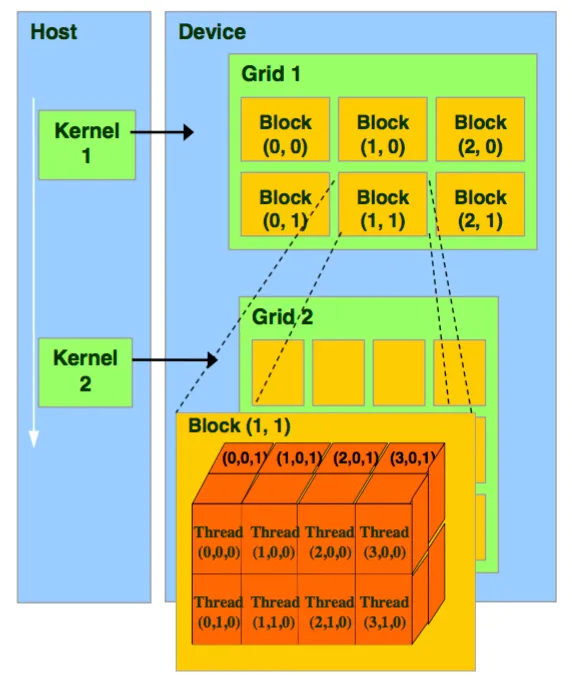
\includegraphics[width=\linewidth]{imagenes/CUDA-blocks-grids.png}
	\caption{Grids y bloques CUDA \cite{Casas2024} }
	\label{fig:CUDA-blocks-grids}
\end{figure}

Como primer ejemplo para ilustrar el modelo, podemos tomar una función auxiliar de la clase \textit{Metodo} como la que ya vimos implementada en OpenMP (algoritmo \ref{alg:VectorCopia-OMP}). En este caso veremos el kernel \textit{escalarPorVector()}. 

\begin{algorithm}[H]
	\begin{algorithmic}
		\State $ i \gets \text{blockDim.x} \cdot \text{blockIdx.x + threadIdx.x} $
		\If{ $ i < N $ }
			\State $ Y[i] \gets Y[i] + X[i] * esc $
		\EndIf
	\end{algorithmic}
	\caption{Kernel escalarPorVector}
	\label{alg:escalarPorVector}
\end{algorithm}

Por un lado, como podemos ver en la primera línea, se calcula un valor $i$ que es igual a una multiplicación y una suma. Identificando a esos 3 elementos tenemos primero a \textit{blockDim.x}, que es un valor igual al tamaño de la dimensión X del bloque al que pertenezca cada thread particular. Luego, \textit{blockIdx.x} designa al bloque individual que contenga cada thread que ejecute el kernel, y de igual manera \textit{threadIdx.x} será el identificador individual de cada thread dentro de su bloque. Combinando los 3 generamos un identificador único para cada uno de los threads que genere el grid.

Por otro lado, se hace la comprobación de que el identificador del thread es menor que el tamaño de los vectores para evitar posibles accesos erróneos a memoria. Esto ha de hacerse ya que, si tenemos un tamaño de problema N, se generará un grid con tantos bloques de tamaño \textit{blockDim.x} como para que el total de hebras sea siempre mayor o igual a N. Dicho de otra forma, con un tamaño de bloque de 256, y un tamaño de problema de 1000, se generaría una grid con 4 bloques (y por tanto 1024 hebras), y las últimas 24 no trabajarían.